% This LaTeX was auto-generated from MATLAB code.
% To make changes, update the MATLAB code and export to LaTeX again.

\documentclass{article}

\usepackage[utf8]{inputenc}
\usepackage[T1]{fontenc}
\usepackage{lmodern}
\usepackage{graphicx}
\usepackage{color}
\usepackage{hyperref}
\usepackage{amsmath}
\usepackage{amsfonts}
\usepackage{epstopdf}
\usepackage[table]{xcolor}
\usepackage{matlab}

\sloppy
\epstopdfsetup{outdir=./}
\graphicspath{ {./parte2_images/} }

\begin{document}

\matlabtitle{II. Equilibrio general}

\begin{par}
\begin{flushleft}
Ahora resolveremos el problema del pescador endogenizando los precios de la economía. Para ello asumiremos que la productividad marginal del trabajo está dada por
\end{flushleft}
\end{par}

\begin{par}
$$\omega =\frac{\partial }{\partial L}F\left(K,L\right)=\left(1-\alpha \right)\;{\left\lbrack \frac{K}{\bar{\;L} }\right\rbrack }^{\alpha }$$
\end{par}

\matlabheading{f. Demostración de  la demanda por capital K y el salario $\omega$ están dados por:}

\begin{par}
$$\begin{array}{l}
K={\left(\frac{\alpha }{r+\delta }\right)}^{\frac{1}{1-\alpha }} \cdot \bar{L} \;\;\;\;\;\;\;\;\;\;\;\;\;\;\;\;\;\;\;\;\;\;\;\;\;\;\;\;\;\;\;\;\;\;\;\;\left(1\right)\\
\omega =\left(1-\alpha \right){\left(\frac{\alpha }{r+\delta }\right)}^{\frac{\alpha }{1-\alpha }} \;\;\;\;\;\;\;\;\;\;\;\;\;\;\;\;\;\;\;\;\;\;\;\;\;\;\;\;\;\left(2\right)
\end{array}$$
\end{par}

\begin{par}
\begin{flushleft}
Primero, debemos partir encontrando las condiciones de primer orden de la función de beneficio. 
\end{flushleft}
\end{par}

\begin{par}
$$\begin{array}{l}
\textrm{Sabemos}\;\textrm{que}\;\textrm{la}\;\textrm{función}\;\textrm{de}\;\textrm{producción}\;\textrm{es}\;\;F\left(K,L\right)=K^{{\;}^{\alpha } } L^{{\;}^{1-\alpha } } ,p\;\textrm{el}\;\textrm{precio}\;\textrm{del}\;\textrm{bien}\;\textrm{que}\;\textrm{las}\;\textrm{empresas}\;\textrm{venden}\;\left(p=1\right),L\;\textrm{el}\;\textrm{empleo},w\;\textrm{el}\;\textrm{salario},K\;\textrm{el}\;\textrm{capital}\;y\;R=\left(r+\delta \right)\;\textrm{su}\;\textrm{costo}\;\textrm{de}\;\textrm{uso}\\
\\
\;\;\;\;\;\;\;\;\;\;\;\;\;\;\;\;\;\;\;\;\;\;\;\;\;\;\;\;\;\;\;\;\;\;\;\;\;\;\;\;\;\;\;\;\;\;\;\;\;\;\;\;\;\;\;\;\;\;\Pi \left(p,w,r,\delta \right)=\max_{K,L} \;\;p\cdot \;F\left(K,L\right)-\left(\omega \cdot L+\left(r+\delta \right)K\right)
\end{array}$$
\end{par}

\begin{par}
$$\begin{array}{l}
{\textrm{PMG}}_k \equiv \frac{\partial }{\partial K}\Pi =\alpha \;{\left(\frac{L}{K}\right)}^{1-\alpha } -\left(r+\delta \right)=0\\
{\textrm{PMG}}_L \equiv \frac{\partial }{\partial L}\Pi =\left(1-\alpha \right)\cdot {\left(\frac{K}{L}\right)}^{\alpha } -\omega =0
\end{array}$$
\end{par}

\begin{par}
\begin{flushleft}
Despejando ${\textrm{PMG}}_k$ obtenemos que
\end{flushleft}
\end{par}

\begin{par}
$$\begin{array}{l}
\alpha \;{\left(\frac{L}{K^* }\right)}^{1-\alpha } =\;\left(r+\delta \right)\leftrightarrow {\left(K^* \right)}^{1-\alpha } =\alpha \;{\left(L\right)}^{1-\alpha } \cdot \left(r+\delta \right)\leftrightarrow K^* =L\cdot {\left(\frac{\alpha }{r+\delta }\right)}^{\frac{1}{1-\alpha }} \\
\;\Rightarrow K^* =L\cdot {\left(\frac{\alpha }{r+\delta }\right)}^{\frac{1}{1-\alpha }} \\

\end{array}$$
\end{par}

\begin{par}
\begin{flushleft}
Tomemos $K^*$ y ingresémoslo a la condición de optimalidad del trabajo
\end{flushleft}
\end{par}

\begin{par}
$$\left(1-\alpha \right)\cdot {\left(\frac{K}{L}\right)}^{\alpha } =\omega \leftrightarrow \left(1-\alpha \right)\cdot \left(\frac{K^* }{L}\right)=\omega \leftrightarrow \omega =\left(1-\alpha \right)\cdot {\left(\frac{L\cdot {\left(\frac{\alpha }{r+\delta }\right)}^{\frac{1}{1-\alpha }} }{L}\right)}^{\alpha }$$
\end{par}

\begin{par}
\begin{flushleft}
Simplifcando llegaremos a que
\end{flushleft}
\end{par}

\begin{par}
$$\Rightarrow \omega =\left(1-\alpha \right)\cdot {\left(\frac{\alpha }{r+\delta }\right)}^{\frac{\alpha }{1-\alpha }}$$
\end{par}

\matlabheading{g. Resolución numérica con función \textit{fisher}}

\begin{par}
\begin{flushleft}
La función \textit{fisher} entrega como output la resolución numérica del agente y recibe como inputs parámetros tales como $r$. En nuestro caso  $\omega$ está definido dentro de la función, dado que su forma funcional no cambia de un ejercicio a otro.  Para responder esta pregunta asumiremos que el salario está dado por la ecuación (2), la oferta laboral de los agentes de edad $t$ es\textbf{ inelástica} y la productividad laboral $\gamma \left(t\right)$ se distribuye normal con media  $\log \left(32\ldotp 5\right)$y desviación estándar  $0\ldotp 4$.
\end{flushleft}
\end{par}

\begin{par}
$$\gamma \left(t\right)=\frac{40}{0\ldotp 4t\sqrt[]{2\pi }}\cdot e{\;}^{\left\lbrack -\frac{1}{2}{\left(\frac{\log \left(t\right)-\log \left(32\ldotp 5\right)}{0\ldotp 4}\right)}^2 \right\rbrack } +0\ldotp 4$$
\end{par}

\begin{par}
\begin{flushleft}
Además, la oferta laboral agregada es una función de la productividad laboral y está dada por
\end{flushleft}
\end{par}

\begin{par}
$$\bar{L} =\sum_{t=1}^T m_t \;\gamma_{t+1}$$
\end{par}

\begin{par}
\begin{flushleft}
De manera más concreta \textit{fisher (3) }es una función que necesita como argumento el horizonte de tiempo del agente, su aversión al riesgo, factor de impaciencia, tasa de interés y restricción de liquidez. Como resultado se obtiene la función de valor, las funciones de política del consumo y capital, las trayectorias del agente en términos del consumo, activos, ahorros y salario. 
\end{flushleft}
\end{par}

\begin{par}
$$\left\lbrack \textrm{vt},\textrm{Api},\textrm{Apf},\textrm{Cpf},\textrm{lt}\_\textrm{activos},\textrm{lt}\_\textrm{consumo},\textrm{lt}\_\textrm{ahorro},\textrm{gamma},y\right\rbrack =\textrm{fisher}\left(T,\textrm{sigma},\textrm{beta},r,h\right)\;\;\;\;\;\;\;\;\;\;\;\;\;\;\;\;\;\;\;\;\;\;\;\;\;\;\;\;\;\;\;\left(3\right)$$     
\end{par}

\begin{par}
\begin{flushleft}
De manera adicional, se ha creado la función \textit{figurepolicy} que permite obtener gráficas para la resolución numérica de los primeros tres resultados de \textit{fisher. }En caso de dudas, para ambas funciones se puede indicar en la consola \textit{help fisher} y aparecerá una ayuda para su uso. 
\end{flushleft}
\end{par}

\matlabheading{h. Oferta agregada de activos \textit{A} y demanda agregada de capital \textit{K}}

\begin{par}
\begin{flushleft}
Ahora analizaremos qué pasa en la economía, a nivel agregado. Para ello definiremos la oferta agregada de activos $\left(A\right)$y la demanda agregada de capital $\left(K\right)$ como 
\end{flushleft}
\end{par}

\begin{par}
\begin{flushleft}
$A=\sum_{t=1}^T m_t \;a_{t+1}$ , 
\end{flushleft}
\end{par}

\begin{par}
$$K={\left(\frac{\alpha }{r+\delta }\right)}^{\frac{1}{1-\alpha }} \cdot \;$$$$\bar{L} ={\left(\frac{\alpha }{r+\delta }\right)}^{\frac{1}{1-\alpha }} \;\cdot \;\sum_{t=1}^T m_t \;\gamma_{t+1}$$
\end{par}

\begin{par}
\begin{flushleft}
Además, en este caso la masa de crecimiento poblacional está definida como $m_t =\frac{1}{T}$, por lo que
\end{flushleft}
\end{par}

\begin{par}
\begin{flushleft}
$A=\frac{1}{T}\sum_{t=1}^T \;a_{t+1}$ , 
\end{flushleft}
\end{par}

\begin{par}
$$K={\left(\frac{\alpha }{r+\delta }\right)}^{\frac{1}{1-\alpha }} \cdot \frac{1}{T}\sum_{t=1}^T \;\gamma_{t+1}$$
\end{par}

\begin{par}
\begin{flushleft}
Como resultado obtenemos la figura 2.1, que contiene al lado izquierdo y derecho respectivamente
\end{flushleft}
\end{par}

\begin{enumerate}
\setlength{\itemsep}{-1ex}
   \item{\begin{flushleft} La trayectoria de activos óptima para cada tasa de interés comprendida en el vector $r\left\lbrack 0,0\ldotp 1\right\rbrack$.  \end{flushleft}}
   \item{\begin{flushleft} La oferta agregada de activos A y la demanda agregada de capital K en función de un vector de tasa de interés $r{\left\lbrack 0,0\ldotp 1\right\rbrack }_{1\textrm{x10}}$ \end{flushleft}}
\end{enumerate}

\begin{par}
\begin{flushleft}
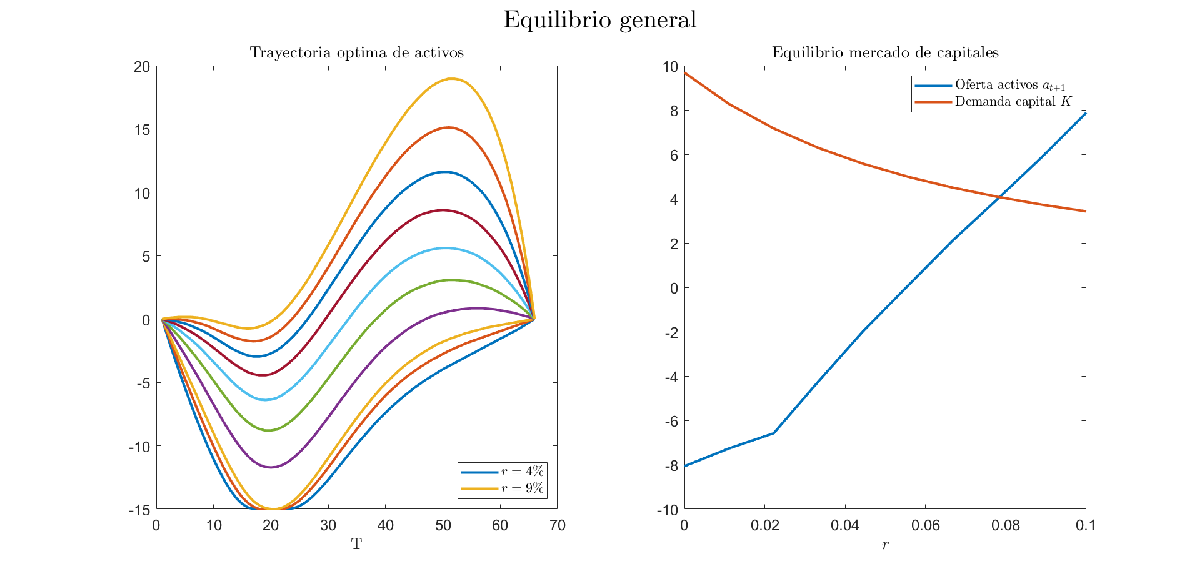
\includegraphics[width=\maxwidth{91.21926743602609em}]{image_0}
\end{flushleft}
\end{par}

\begin{par}
\begin{center}
Figura E. Equilibrio general sin restricciones
\end{center}
\end{par}

\begin{par}
\begin{flushleft}
En la figura de la izquierda tenemos en el eje \textit{y el nivel de activos } y en el eje \textit{X }los periodos de ciclo de vida del agente. Por ello, en general, el agente en los primeros periodos de ciclo de vida se endeuda (\textit{nivel de activos negativos}) hasta aproximadamente el periodo 20, y luego comienza a acumular activos hasta aproximadamente el periodo 50, donde estos se vuelven a gastar hasta quedar con 0 nivel de activos en el último periodo. Como comentamos en el inciso anterior, esta trayectoria se condice con lo indicado por la teoría de la renta permanente que indica que los agentes deciden su trayectoria de consumo en base al ingreso esperado para todo el ciclo de vida. Como en los primeros periodos obtenemos un ingreso menor (figura 2.2) el agente para suavizar su consumo accederá a deuda para poder lograr dicho objetivo. Así, a medida que mejora la trayectoria salarial, la necesidad de acceso al crédito disminuye incluso llegando a poder ahorrar. Ahora bien, lo distintivo que aporta esta gráfica es que mientras menor es la tasa de interés (línea azul) mayor es la deuda a la que acceden los agentes, a diferencia de tasas que bordean el 1\% (línea amarilla). Este resultado es totalmente esperable toda vez que la tasa de interés corresponde al precio del crédito, por lo que su acceso para lograr el objetivo de suavizar consumo (en ausencia de restricciones financieras) es logrado de manera más holgada en contextos de baja tasa de interés. Una segunda trayectoria a destacar es la que ocurre entre la \textit{línea celeste y roja }pues esta se aproxima a la tasa de interés de equilibrio, es decir, sea que la demanda de activos por activos es cero o bien la oferta por activos es cero.
\end{flushleft}
\end{par}

\begin{par}
\begin{flushleft}
De hecho, gráficamente lo podemos ver en la figura de la derecha que representa la oferta y demanda agregada de activos y capital, respectivamente. No es sorpresivo notar que a una mayor tasa de interés, la oferta de activos aumenta pues los mercados financieros se ven beneficiados en términos de retornos por el aumento del precio de los activos (por ejemplo, bonos). Mientras que por el lado de la demanda, esta tiene una pendiente negativa en relación a un aumento de la tasa de interés. Como se puede ver, donde se intersectan ambos mercados corresponde al punto donde el nivel de activos es cero, a una cierta tasa de interés que llamaremos la \textit{tasa de interés de equilibrio. }Como se puede ver en la figura, este valor esta aproximadamente entre el intervalo 0.06 y 0.08.
\end{flushleft}
\end{par}

\matlabheading{i. Endogenizando $r\;y\;\omega$, encuentre la tasa de equilibrio del mercado de capitales}

\begin{par}
\begin{flushleft}
Para poder encontrar una aproximación puntual a esa tasa de equilibrio ocuparemos el algoritmo de bisección para aproximar la solución. A diferencia del enunciado, no utilizaremos como función objetivo $\frac{A-K}{K}$ pese a que correctamente va comparando la distancia entre ambos mercados para obtener la solución 0. La razón corresponde a la eficiencia: esto implica computar un agregado adicional y luego calcular una función objetivo. De manera alternativa, se utilizará como función objetivo la \textit{oferta agregada de activos }pues, como indicamos arriba, la tasa de interes de equilibrio corresponde a aquella donde la oferta se hace cero (como analizamos para la figura 2.1 de la izquierda y derecha).  Además, existen dos formas de computar el algoritmo de bisección (y ambas llegan al mismo resultado). En la primera se implementa un número entero de 100 iteraciones, además de restringuir la solución sí y solo sí $\rho \;\left(0\ldotp 041\right)\cdot \rho \;\left(0\ldotp 09\right)<0$, pues en caso contrario no se puede asegurar la solución. Como resultado, el algortimo nos dará el punto intermedio del n-ésimo intervalo computado por el método. El segundo método, y que ocuparemos en general para la resolución de la tarea, corresponde a comparar los signos de la función objetivo en el intervalo inferior y la función objetivo evaluada en el intervalo medio, y si son de signo igual se redefine el intervalo inferior en términos del intervalo medio. 
\end{flushleft}
\end{par}

\begin{par}
\begin{flushleft}
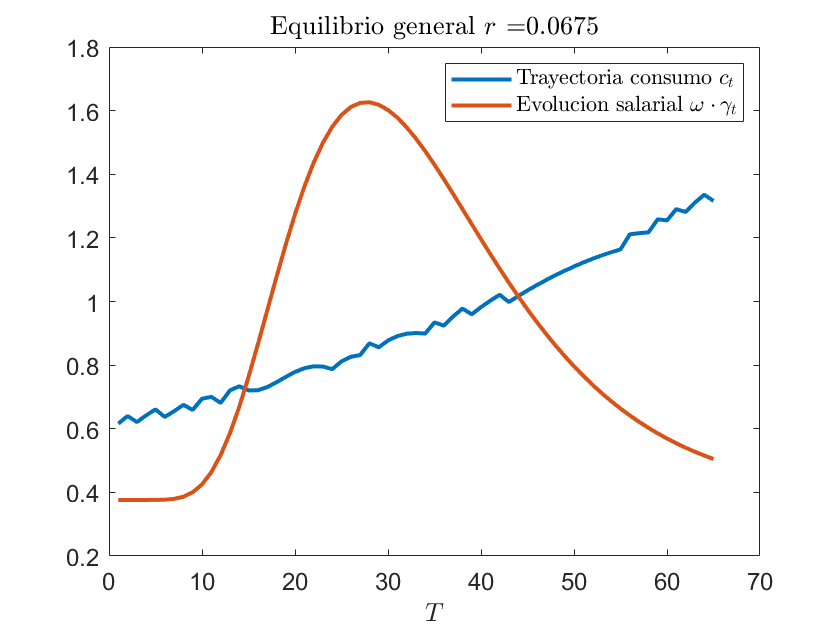
\includegraphics[width=\maxwidth{64.92724535875564em}]{image_1}
\end{flushleft}
\end{par}

\begin{par}
\begin{center}
Figura F. Trayectoria salarial y del consumo en equilibrio
\end{center}
\end{par}

\begin{par}
\begin{flushleft}
Entonces, como se había anticipado en el punto anterior, buscamos encontrar el equilibrio del mercado de capitales donde se iguala la oferta y demanda. Un método puede ser gráficamente, esto es, mirando donde la demanda o la oferta de activos se hacen cero, o bien se intersectan ambas rectas. Otra forma es tomar un intervalo acotado donde sabemos que está la solución, pero no ella exactamente, ir computando la diferencia de las rectas y encontrar cuando estas se hacen cero (o equivalentemente, buscan cuando una de ellas se hace cero), y si no se encuentra dicho valor, volver a acotar el intervalo de estudio. Económicamente tiene sentido pensar que esta tasa es la del equilibrio pues es la situación donde los oferentes de activos (ej. bancos, agentes intermediarios) prestan todos los activos disponibles y los agentes demandantes (ej. hogares) piden todos esos activos pues el precio de los activos maximiza la utilidad para ambos agentes.
\end{flushleft}
\end{par}

\begin{par}
\begin{flushleft}
A partir de la tasa de interés de equilibrio, hemos construido la figura i que representa la trayectoria de consumo (recta azul) y salarial (curva naranja) de los agentes. Como podemos notar, en el equilibrio y en ausencia de fricciones crediticias, el agente puede cumplir su objetivo de suavizar su consumo. ¿Cómo sabemos esto? La razón es que, dado que el agente define su trayectoria de consumo en base a su ingreso esperado se podría esperar que el consumo siguiera la trayectoria del salario, esto es, una distribución normal. Pero, dado que el agente no tiene restricciones crediticias, en la primera parte de su ciclo de vida podrá acceder a deuda para financiar su consumo presente. Además, dado que estamos en un contexto de competencia perfecta, el salario es igual a la productividad marginal del trabajo, por lo que, tal como indican la economía laboral, los periodos de mayor productividad del trabajador es la edad media  (Maestas, Mullen y Powell, 2016), y consecuencia de ello, en estos periodos se podrá ahorrar también para suavizar consumo cuando el salario sea cero o solo se perciban ingresos de las pensiones. La función política del consumo se nota más claramente en la Figura I.A que hemos dejado en los anexos. 
\end{flushleft}
\end{par}

\matlabheading{j. Implicancias de las fricciones financieras sobre la trayectoria de ciclo de vida económica y equilibrio general }

\begin{par}
\begin{flushleft}
En el apartado anterior hicimos la precisión de que el agente logra \textit{suavizar consumo} sujeto a que estamos en ausencia de restricciones financieras. Ahora bien, ¿podemos sostener estos mismos resultados en un contexto de fricciones financieras? Durante los años 60, distintos economistas criticaron la teoría de Friedman sobre todo respecto a los supuestos esbozados respecto a como se proponía que era la función del consumo y cómo era realmente en los datos (cf. Mayer, 1972; cf. Friend y Kravis, 1957). Parte importante de los argumentos residían en que no es posible (1) asumir la propensión marginal a consumir es constante, (2) que la propensión marginal a consumir del ingreso transitorio es cero y que (2) la propensión marginal a consumir es tan baja.  Así y todo, autores como Ando, A., \& Modigliani, F (1963), Hall (1978) y más recientemente, Campbell y Mankiw (1991), salieron al paso de estas críticas haciendo una modificación de la teoría suponiendo que los resultados de Friedman eran ciertos bajo un contexto de fricciones financieras. 
\end{flushleft}
\end{par}

\begin{par}
\begin{flushleft}
Ante ello, el los siguientes dos apartados tomaremos estas ideas para analizar los resultados gráficos de la Figura j, de cómo cambia la (1) la trayectoria de activos óptima, (2) la tasa de interés de equilibrio, (3) la trayectoria de consumo óptima (junto al ingreso) y (4) la correlación consumo-ingreso \textbf{en función de la restricción de liquidez.}
\end{flushleft}
\end{par}

\begin{par}
\begin{flushleft}
En primer lugar, la trayectoria óptima de activos se ve severamente afectada. Por un lado, en ausencia de restricciones los agentes podrán endeudarse en los primeros periodos de su ciclo de vida (curva amarilla decreciente hasta el periodo 20), luego pagar la deuda y ahorrar (curva creciente hasta periodo 50), y luego gastar de esos ahorros para morir sin activos. Por otro lado, a medida que aumentan las restricciones financieras (la máxima expresión es la recta azul), el agente no tendrá menos posibilidades de endeudarse y ahorrar, o en otras palabras, participar del mercado de capitales. Esto es consistente con la trayectoria de consumo: antes habíamos indicado que el agente, gracias al acceso del mercado financiero iba a poder suavizar su consumo (notemos las rectas planas en la figura de la trayectoria de consumo). Ahora, el agente sigue una trayectoria de consumo consistente a su ingreso, y por ello, el resto de las trayectorias de consumo siguen una distribución normal. De modo de simplificar la gráfica, solo se muestra una trayectoria salarial pues esta al ser definida por la tasa de interés de equilibrio (y esta sensible a las restricciones de liquidez), tiene muchas trayectorias posibles pero con la misma distribución (véase la ecuación de $\omega \cdot \gamma \left(t\right)$, donde $\omega$ depende de $r$ y $\gamma \left(t\right)~N\left(\log \left(32\ldotp 5\right),0\ldotp 4\right)$. Con esto último anunciamos un punto relevante, y es que, la tasa de interés de equilibrio se ve afectada por las restricciones de liquidez. A medida que aumentan restricción de liquidez o endeudamiento, la tasa de interés de equilibrio va a aumentar. La intuición es que esto opera directamente como una limitante al acceso del crédito (como analizamos en la trayectoria óptima de activos), es decir, la oferta agregada de activos se va a ver restringuida, y a un mismo nivel de demanda, los precios se los activos van a subir (figura adicional de anexos de como se contrae la oferta). En síntesis, la tasa de interés de equilibrio va a aumentar ante el nuevo equilibrio entre demanda y oferta.
\end{flushleft}
\end{par}

\begin{par}
\begin{flushleft}
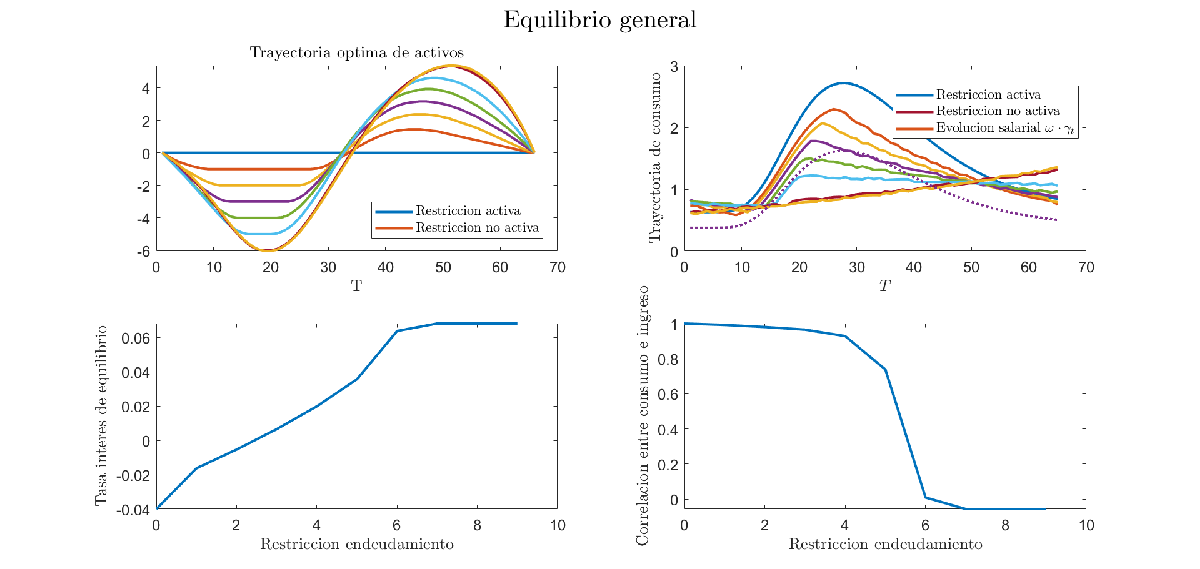
\includegraphics[width=\maxwidth{120.42147516307075em}]{image_2}
\end{flushleft}
\end{par}

\begin{par}
\begin{center}
Figura G. Equilibrio general y trayectorias de ciclo de vida con restricciones
\end{center}
\end{par}

\matlabheading{k. Relación entre consumo e ingreso}


\vspace{1em}
\begin{par}
\begin{flushleft}
Pensemos en las fuentes de financiamiento del consumo: ingresos, ahorro o deuda. Si el agente nace sin activos, su posibilidad de consumo básicamente se define por su nivel salarial y su capacidad de endeudarse (y luego pagar esa deuda). Si el agente no puede endeudarse (restricción de liquidez en 0), entonces el consumo depende plenamente de los ingresos. A medida que la restricción de liquidez se va flexibilizando, el agente podrá acceder a creditos para suavizar consumo. Con ello, la relación entre consumo e ingresos va disminuyendo en su tamaño efecto. Esta relación es muy expresiva de cómo se da la trayectoria de consumo con posibilidad acceder a deuda y sin la posibilidad. En el último caso notaremos, en general, trayectorias de consumo que se asimilan a las del ingreso. Mientras que en contextos con posibilidad de deuda, el agente podrá endeudarse para poder suavizar consumo. Ahora bien, esto podría darse solo en la primera parte de la trayectoria del agente. ¿Por qué? La razón es que, si las preferencias del agente así lo indican ( por ejemplo, podría ser que $r>\rho$), el agente podría decidir ahorrar parte de sus ingresos salariales para consumir mañana (un ahorro autoimpuesto o \textit{buffer stock} planteado por Christopher Carrol en múltiples de sus investigaciones). Así también, podría decidir ahorrar precautoriamente de su salario ante la posibilidad de un ingreso salarial cero al final de su ciclo de vida. En síntesis, la correlación consumo e ingreso también dependerá de la forma funcional del consumo del agente, pues parte de ese consumo factible actual podría ser transferido a consumo factible futuro vía el ahorro. En este caso se da que el agente, en el equilibrio, decidiría ocupar todo de su salario para poder obtener mayor utilidad. 
\end{flushleft}
\end{par}

\begin{par}
\begin{flushleft}
Si la tasa de interés \textit{de equilibrio} fuera más baja, eso implicaría que por el lado de la oferta los mercados están más dispuestos a prestar a una menor tasa de interés, mientras que por el lado de la demanda esta es la tasa máxima a la que están dispuestos los agentes a tomar deuda.Si es que las instituciones bancarias no decidieran poner más límites en términos de restricciones (por ejemplo, requisitos de niveles de ingresos), entonces los agentes tendrán más posibilidad de acceder a crédito en el corto plazo. Pero en el largo plazo, ese bajo precio será el precio que se les paga por sus ahorros. Por lo que, suponiendo que esa baja tasa no corresponde a un shock,  y es totalmente anticipada, entonces la correlación del consumo e ingreso respecto a las restricciones podría bajar en intensidad (nuevamente, manteniendo constante la restricción de liquidez, pensando en el corto plazo y a una tasa de interés esperada). 
\end{flushleft}
\end{par}

\begin{par}
\begin{flushleft}
Nos gustaría cerrar este apartado aportando con el análisis de Carrol respecto a la relación entre ingresos y consumo. Como analiza Carrol (2001), a medida que la riqueza se vuelve más grande, la pendiente del consumo en tiempo infinito se vuelve cada vez más similar a la pendiente del consumo con \textit{perfect foresight. }Esto es, como la riqueza (por ejemplo, medida en ingresos) se vuelve muy grande, la propensión marginal a consumir es la misma que en un enfoque de horizonte perfecto sin incertidumbre. La razón de porqué ocurre esto que es dado que la riqueza es muy grande (wealth approches infinity), la proporción de \textbf{consumo futuro }que debería ser financiada con fondos que serán \textbf{inciertos} hace que esa \textbf{incertidumbre sea irrelevante para la decisión del consumo. }Si bien en este caso no analizamos el efecto de la incertidumbre en la decisión, si podemos hipotetizar que si extendemos este análisis para infinitos periodos es probable que esta relación positiva y fuerte entre consumo e ingreso siga siendo robusta, independiente de todos los \textit{peros }que pusimos a lo largo del análisis. 
\end{flushleft}
\end{par}

\matlabheading{Referencias}

\begin{par}
\begin{flushleft}
Ando, A., \& Modigliani, F. (1963). The" life cycle" hypothesis of saving: Aggregate implications and tests. \textit{The American economic review}, \textit{53}(1), 55-84
\end{flushleft}
\end{par}

\begin{par}
\begin{flushleft}
Campbell, J. Y., \& Mankiw, N. G. (1991). The response of consumption to income: a cross-country investigation. \textit{European economic review}, \textit{35}(4), 723-756.
\end{flushleft}
\end{par}

\begin{par}
\begin{flushleft}
Friedman, M. (1957). The permanent income hypothesis. In \textit{A theory of the consumption function} (pp. 20-37). Princeton University Press.
\end{flushleft}
\end{par}

\begin{par}
\begin{flushleft}
Friend, I., \& Kravis, I. B. (1957). Consumption patterns and permanent income. \textit{The American Economic Review}, \textit{47}(2), 536-555.
\end{flushleft}
\end{par}

\begin{par}
\begin{flushleft}
Hall, R. E. (1978). Stochastic implications of the life cycle-permanent income hypothesis: theory and evidence. \textit{Journal of political economy}, \textit{86}(6), 971-987.
\end{flushleft}
\end{par}

\begin{par}
\begin{flushleft}
Maestas, N., Mullen, K. J., \& Powell, D. (2016). \textit{The effect of population aging on economic growth, the labor force and productivity} (No. w22452). National Bureau of Economic Research.
\end{flushleft}
\end{par}

\begin{par}
\begin{flushleft}
Mayer, T. (1972). Permanent income, wealth, and consumption. In \textit{Permanent Income, Wealth, and Consumption}. University of California Press.
\end{flushleft}
\end{par}

\end{document}
